\chapter{dials buttons switches} 
\label{sec:dials}
\begin{definition}[Jeffrey Says\index{Jeffrey Says}]
\setlength{\intextsep}{0pt}%
\setlength{\columnsep}{3pt}%
\begin{wrapfigure}{l}{0.12\textwidth}

\includegraphics[width=\linewidth]{src/callout/psych.png} 
\end{wrapfigure}
\small
Gradually the idea solidified into the concept of a
light-show generator, something interactive, creative but simple
enough so that anyone could do it, yet complex enough to produce
breathtaking results once learned well. A program to do for light, in
fact, what a synthesiser does for sound.
\end{definition}

Dials, buttons, switches, and knobs that we can twiddle and adjust are at the heart of the 
Psychedelia player's experience. Fortunately they are mostly packaged up into presets and bursts,
as we have already seen. However it is possible, if you are prepared to clutch the game's manual
to your chest at night in bed, to configure many individual settings in all sorts of different ways.

In this penultimate chapter we'll take a look at the more interesting of these settings in some detail, develop
a better idea of how they are supposed to work, and figure out how they were incorporated into the core routines
we covereded in earlier chapters.

\begin{figure}[H]
    \centering
    \begin{adjustbox}{width=3cm,margin=11cm -12cm}
      
\includegraphics[width=12cm]{src/delay/delay-low.png}%
    \end{adjustbox}
    \begin{adjustbox}{width=10.5cm,center}
      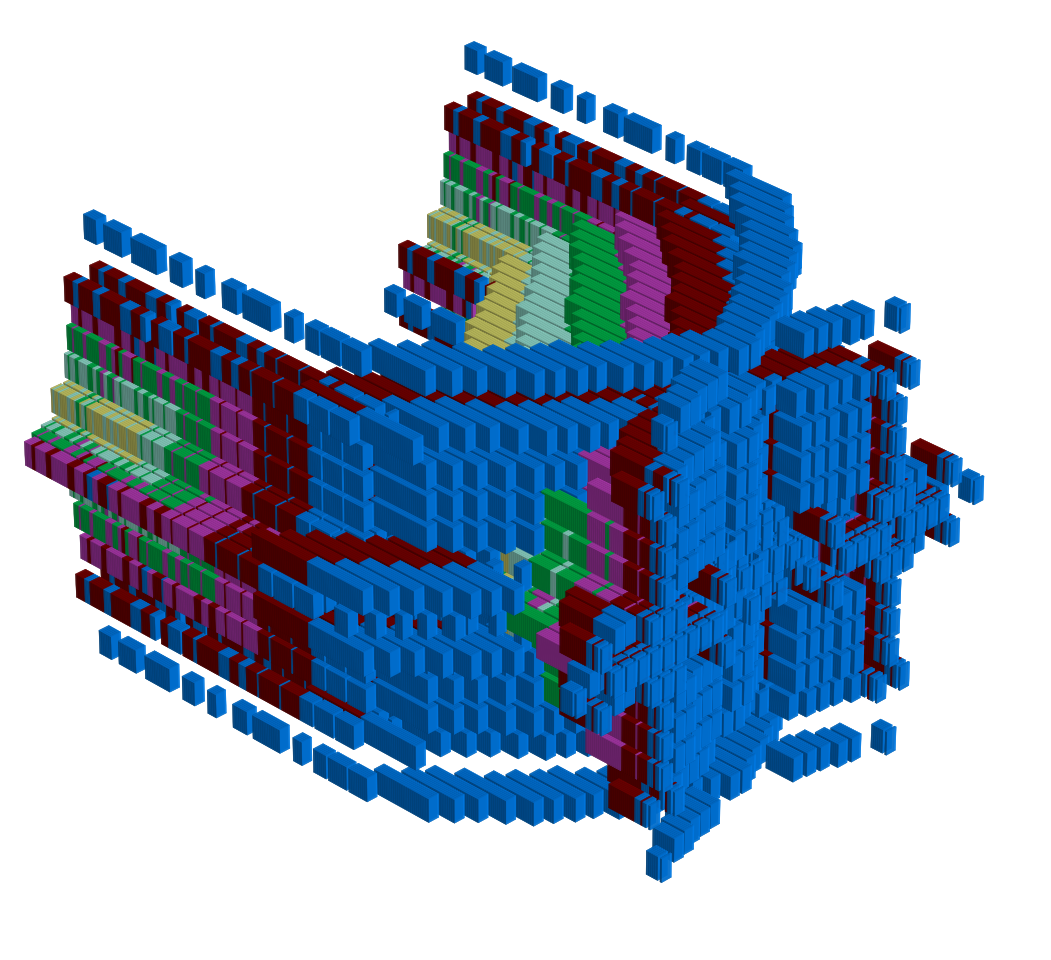
\includegraphics[width=12cm]{src/delay/pattern0-45.png}%
    \end{adjustbox}
    \begin{adjustbox}{width=3cm,margin=11cm -12cm}
      
\includegraphics[width=12cm]{src/delay/delay-high.png}%
    \end{adjustbox}
    \begin{adjustbox}{width=10.5cm,margin=0cm -2cm}
      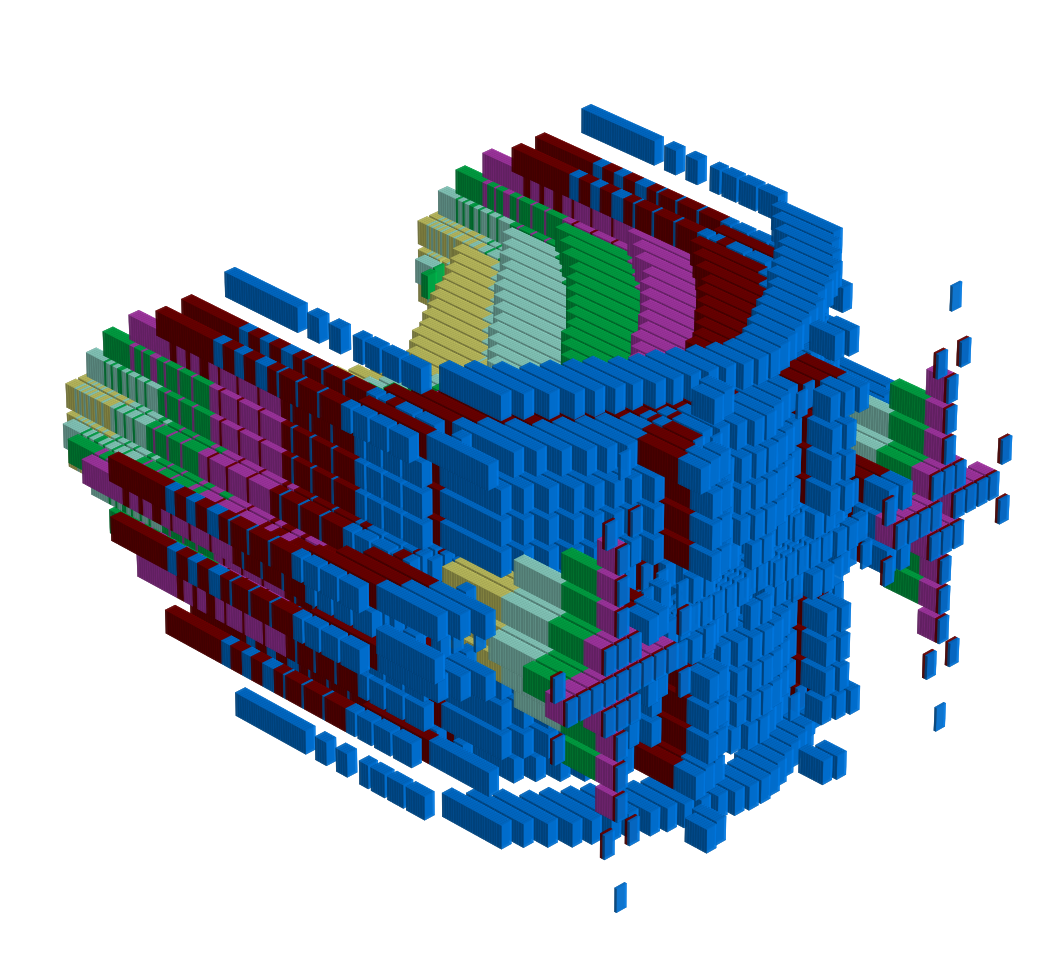
\includegraphics[width=12cm]{src/delay/pattern1-45.png}%
    \end{adjustbox}
    \caption{Effect of low and high values for Smoothing Delay}
\end{figure}
\clearpage

\section*{smoothing delay} 
\label{sec:delay}
\lstset{style=6502Style}
\lstset{ 
   aboveskip=5pt,
   belowskip=0pt,
}

\begin{definition}[Jeffrey Says\index{Jeffrey Says}]
\setlength{\intextsep}{0pt}%
\setlength{\columnsep}{3pt}%
\begin{wrapfigure}{l}{0.12\textwidth}

\includegraphics[width=\linewidth]{src/callout/psych.png} 
\end{wrapfigure}
\small
\textbf{D to activate:} Because of the time taken to
draw larger patterns speed increase/decrease is not linear. You
can adjust the ‘compensating delay’ which often smooths out jerky
patterns. Can be used just for special FX, though. Suck it and see.
\end{definition}

So that's clear then. Smoothing delay is what you want to use when
you need to smooth out the delay. What more explanation could we need?

If we look at the effect of setting this parameter to its lowest and
highest possible value opposite, the difference in behaviour is not
extreme. It's almost quite subtle. With a higher setting the pattern
evolves in a more drawn out fashion - as though a higher value lets
Psychedelia linger a little longer on the current state of the pattern
rather than immediately evolving it to the next state.

Let's dig into the code and see if this intuition is correct.

First of all though we'll take a look at the code that allows us to
twiddle this:

    \begin{adjustbox}{width=9cm}
      \frame{
\includegraphics[width=12cm]{src/delay/delay-low.png}}%
    \end{adjustbox}

to this:

    \begin{adjustbox}{width=8.2cm}
      \frame{
\includegraphics[width=12cm]{src/delay/delay-high.png}}%
    \end{adjustbox}

\clearpage

\textbf{Lines 1297-1303. \icode{\textbf{MaybeDPressed}}}
\begin{lstlisting}[caption=From \icode{CheckKeyboardInput\index{CheckKeyboardInput}}.,escapechar=\%]
MaybeDPressed   
        CMP #KEY_D ; 'D' pressed?
        BNE MaybeCPressed

DPressed
        LDA #$01
        STA currentVariableMode%\index{currentVariableMode}%
        RTS 
\end{lstlisting}
\textbf{Lines 1838-1868. \icode{\textbf{UpdateVariableDisplay}}}
\begin{lstlisting}[caption=From \icode{CheckKeyboardInputForActiveVariable}.,escapechar=\%]
UpdateVariableDisplay   
        ...

        LDX currentVariableMode%\index{currentVariableMode}%
        LDA lastKeyPressed%\index{lastKeyPressed}%
        CMP #KEY_GT ; > pressed?
        BNE MaybeLeftArrowPressed

RightArrowPressed
        ; > pressed, increase the value bar.
        INC presetValueArray%\index{presetValueArray}%,X
        LDA presetValueArray%\index{presetValueArray}%,X
        ; Make sure we don't exceed the max value.
        CMP maxValueForPresetValueArray,X
        BNE MaybeInColorMode%\index{MaybeInColorMode}%
        DEC presetValueArray%\index{presetValueArray}%,X
        JMP MaybeInColorMode%\index{MaybeInColorMode}%

MaybeLeftArrowPressed   
        CMP #KEY_LT ; < pressed?
        BNE MaybeInColorMode%\index{MaybeInColorMode}%

        ; < pressed, decrease the value bar.
        DEC presetValueArray%\index{presetValueArray}%,X
        LDA presetValueArray%\index{presetValueArray}%,X
        ; Make sure we don't exceed the min value.
        CMP minValueForPresetValueArray,X
        BNE MaybeInColorMode%\index{MaybeInColorMode}%
        INC presetValueArray%\index{presetValueArray}%,X

\end{lstlisting}
\clearpage
\textbf{Lines 1297-1303. \icode{\textbf{MaybeDPressed}}:} When \icode{D} is pressed we don't
update a setting there and then as you might expect. Instead we get ready to display the 'Smoothing
Delay' control bar, by... loading the value \icode{\$01} to \icode{currentVariableMode\index{currentVariableMode}}? Okay, we'll
go with that for now.

\textbf{Lines 1838-1868. \icode{\textbf{UpdateVariableDisplay}}:}  The next time we loop around
to \icode{Check\-KeyboardInput}, we hit this little piece of logic at the very top of it:

\begin{lstlisting}[escapechar=\%]
CheckKeyboardInput%\index{CheckKeyboardInput}%   
        LDA currentVariableMode%\index{currentVariableMode}%
        BEQ CheckForGeneralKeystrokes
        JMP CheckKeyboardInputForActiveVariable
\end{lstlisting}

Well, we just loaded \icode{\$01} to \icode{currentVariableMode\index{currentVariableMode}} above so it's not zero.  It follows that
the \icode{BEQ} check will give a negative result (the check means 'is the value in \icode{A} equal to zero?'), 
so instead of forking to \icode{CheckForGeneralKeystrokes} we'll \icode{JMP} to \icode{CheckKeyboardInputForActiveVariable}.

This is where the function we're looking at here lives. As we can see the first thing it does is load 
\icode{currentVariableMode\index{currentVariableMode}} to the \icode{X} register. This is because we're going to use it as an index
into an array we encountered in the previous chapter on Presets. This is the array \icode{presetValueArray\index{presetValueArray}}
which contains a lot of the settings we'll be looking at in this chapter huddled together like a gaggle
of ducklings, with \icode{smoothingDelay\index{smoothingDelay}} near the head at index 1 (index 0 being taken by \icode{unusedPresetByte}):

\begin{lstlisting}[escapechar=\%]
presetValueArray%\index{presetValueArray}%
unusedPresetByte        .BYTE $00
smoothingDelay%\index{smoothingDelay}%          .BYTE $0C
cursorSpeed             .BYTE $02
bufferLength%\index{bufferLength}%            .BYTE $1F
pulseSpeed              .BYTE $01
...
\end{lstlisting}

With \icode{X} set to 1 we can now use it increment the value for \icode{smoothingDelay\index{smoothingDelay}} by
simply executing:
\begin{lstlisting}[escapechar=\%]
        INC presetValueArray%\index{presetValueArray}%,X
\end{lstlisting}
And decrement it by doing:
\begin{lstlisting}[escapechar=\%]
        DEC presetValueArray%\index{presetValueArray}%,X
\end{lstlisting}
This is handy, and worth remembering as the technique will be reused for adjusting other values that 
we look at that also live in \icode{presetValueArray\index{presetValueArray}}.

\clearpage

\textbf{Lines 923-928. \icode{\textbf{ApplySmoothingDelay}}}
\begin{lstlisting}[caption=From \icode{MainInterruptHandler}.,escapechar=\%]
ApplySmoothingDelay    
        LDA smoothingDelay%\index{smoothingDelay}%
        STA initialSmoothingDelayForStep,X
        STA smoothingDelayForStep,X
\end{lstlisting}
\textbf{Lines 644-679. \icode{\textbf{ShouldDoAPaint}}}
\begin{lstlisting}[caption=From \icode{MainPaintLoop\index{MainPaintLoop}}.,escapechar=\%]
ShouldDoAPaint   
        ...
        DEC smoothingDelayForStep,X
        BNE GoBackToStartOfLoop

        ; Actually paint some pixels to the screen.
        ; Reset the delay for this step.
        LDA initialSmoothingDelayForStep,X
        STA smoothingDelayForStep,X

        ; Get the x and y positions for this pixel.
        LDA pixelXPositionArray%\index{pixelXPositionArray}%,X
        STA pixelXPositionZP
        LDA pixelYPositionArray%\index{pixelYPositionArray}%,X
        STA pixelYPositionZP

        LDA patternIndexArray%\index{patternIndexArray}%,X
        STA presetIndex

        LDA symmetrySettingForStepCount%\index{symmetrySettingForStepCount}%,X
        STA currentSymmetrySettingForStep%\index{currentSymmetrySettingForStep}%

        LDA currentIndexToColorValues
        AND #$80
        BNE ResetAndGoBackToStartOfLoop

        TXA 
        PHA 
        JSR PaintStructureAtCurrentPosition
        PLA 
        TAX 
\end{lstlisting}
\clearpage

\textbf{Lines 923-928. \icode{\textbf{ApplySmoothingDelay}}:} With the player's selected value loaded 
safely to \icode{smoothingDelay\index{smoothingDelay}} we now have to see how it is applied to the evolution of the patterns.

The immediate answer to this is given here: it is loaded to the current position in the 
\icode{smoothingDelayForStep} and \icode{initialSmoothingDelayForStep} arrays. Remember that these
arrays, along with several others, help track the different phases in the evolution of the pattern.


\textbf{Lines 644-679. \icode{\textbf{ShouldDoAPaint}}:}  Back to the main paint loop, where the
pixel painting is actually done. We looked at this loop in detail in earlier chapters. And it is in
here that we see the 'smoothing delay' get applied. At the top of function we've extracted here
the value in \icode{smoothingDelayForStep} is used as a countdown counter. This is what our
smoothing delay is: a counter that we decrement at each pass. If it's not zero yet (\icode{BNE}),
we \icode{GoBackToStartOfLoop}.

If it is zero we can actually paint a pixel. We use the value in \icode{initialSmoothing\-DelayForStep}
to reset our counter and get on with doing a full paint.

So after all that we can see that 'smoothing delay' acts as a brake on the painting loop - the greater
the value the longer it will defer the next paint, resulting in a slower and smoother evolution of the
pattern being painted.

